\documentclass{article}

\usepackage{fancyhdr}
\usepackage{extramarks}
\usepackage{amsmath}
\usepackage{amsthm}
\usepackage{amsfonts}
\usepackage{tikz}
\usepackage[plain]{algorithm}
\usepackage{algpseudocode}
\usepackage{enumerate}
\usepackage{graphicx}
\usepackage{pythonhighlight}
\usepackage{amssymb}

\usetikzlibrary{automata,positioning}

%
% Basic Document Settings
%  

\topmargin=-0.45in
\evensidemargin=0in
\oddsidemargin=0in
\textwidth=6.5in
\textheight=9.0in
\headsep=0.25in

\linespread{1.1}

\pagestyle{fancy}
\lhead{\hmwkAuthorName}
\chead{\hmwkClass\ (\hmwkClassInstructor): \hmwkTitle}
\rhead{\firstxmark}
\lfoot{\lastxmark}
\cfoot{\thepage}

\renewcommand\headrulewidth{0.4pt}
\renewcommand\footrulewidth{0.4pt}

\setlength\parindent{0pt}

%
% Create Problem Sections
%

\newcommand{\enterProblemHeader}[1]{
    \nobreak\extramarks{}{Problem \arabic{#1} continued on next page\ldots}\nobreak{}
    \nobreak\extramarks{Problem \arabic{#1} (continued)}{Problem \arabic{#1} continued on next page\ldots}\nobreak{}
}

\newcommand{\exitProblemHeader}[1]{
    \nobreak\extramarks{Problem \arabic{#1} (continued)}{Problem \arabic{#1} continued on next page\ldots}\nobreak{}
    \stepcounter{#1}
    \nobreak\extramarks{Problem \arabic{#1}}{}\nobreak{}
}

\setcounter{secnumdepth}{0}
\newcounter{partCounter}
\newcounter{homeworkProblemCounter}
\setcounter{homeworkProblemCounter}{1}
\nobreak\extramarks{Problem \arabic{homeworkProblemCounter}}{}\nobreak{}

%
% Homework Problem Environment
%
% This environment takes an optional argument. When given, it will adjust the
% problem counter. This is useful for when the problems given for your
% assignment aren't sequential. See the last 3 problems of this template for an
% example.
%
\newenvironment{homeworkProblem}[1][-1]{
    \ifnum#1>0
        \setcounter{homeworkProblemCounter}{#1}
    \fi
    \section{Problem \arabic{homeworkProblemCounter}}
    \setcounter{partCounter}{1}
    \enterProblemHeader{homeworkProblemCounter}
}{
    \exitProblemHeader{homeworkProblemCounter}
}

%
% Homework Details
%   - Title
%   - Due date
%   - Class
%   - Section/Time
%   - Instructor
%   - Author
%

\newcommand{\hmwkTitle}{Homework\ \#3}
\newcommand{\hmwkDueDate}{April 16, 2020}
\newcommand{\hmwkClass}{Reinforcement Learning}
\newcommand{\hmwkClassInstructor}{Professor Ziyu Shao}
\newcommand{\hmwkAuthorName}{Tianyuan Wu}
\newcommand{\hmwkAuthorID}{63305667}

%
% Title Page
%

\title{
    \vspace{2in}
    \textmd{\textbf{\hmwkClass:\ \hmwkTitle}}\\
    \normalsize\vspace{0.1in}\small{Due\ on\ \hmwkDueDate\ at 11:59pm}\\
    \vspace{0.1in}\large{\textit{\hmwkClassInstructor}}
    \vspace{3in}
}

\author{\textbf{\hmwkAuthorName}\\ \hmwkAuthorID}
\date{}

\renewcommand{\part}[1]{\textbf{\large Part \Alph{partCounter}}\stepcounter{partCounter}\\}

%
% Various Helper Commands
%

% Useful for algorithms
\newcommand{\alg}[1]{\textsc{\bfseries \footnotesize #1}}

% For derivatives
\newcommand{\deriv}[1]{\frac{\mathrm{d}}{\mathrm{d}x} (#1)}

% For partial derivatives
\newcommand{\pderiv}[2]{\frac{\partial}{\partial #1} (#2)}

% Integral dx
\newcommand{\dx}{\mathrm{d}x}

% Alias for the Solution section header
\newcommand{\solution}{\textbf{\large Solution}}

% Probability commands: Expectation, Variance, Covariance, Bias
\newcommand{\E}{\mathrm{E}}
\newcommand{\Var}{\mathrm{Var}}
\newcommand{\Cov}{\mathrm{Cov}}
\newcommand{\Bias}{\mathrm{Bias}}

\begin{document}

\maketitle

\pagebreak

\begin{homeworkProblem}
    \textbf{Solution}
    \begin{enumerate}[a]
        \item[a)]
            Because the initial state $X_0$ follows the stationary distribution, 
            for every state $X_i$, the marginal distribution is $s$. i.e. $\forall n\in N, P(X_n=i)=s_i$.
            In this case, there are 10 states, and $P(X_n=3) = s_3$. So, on average, the number of states 
            in $X_0, \ldots, X_9$ equals to $3$ is $10s_3$.
        \item[b)]
            In this case, it's obviously that if $X_n=1$ or $X_n=2$, then $Y_n=0$, and if $X_n=3$, then $Y_n=2$.
            It means, we have `merged' state space $1$ and $2$ to $0$.  So if we make the transition matrix $Q$ be:
            \begin{equation}\nonumber
                Q= 
                \begin{bmatrix} 
                    \frac{1}{3} & \frac{1}{3} & \frac{1}{3} \\ 
                    \frac{1}{3} & \frac{1}{3} & \frac{1}{3} \\
                    \frac{1}{3} & \frac{1}{3} & \frac{1}{3}
                \end{bmatrix}
            \end{equation}
            The Markov property holds.
            But if we put $Q$ be the following form, $Y_n$ is not Markov.
            \begin{equation}\nonumber
                Q= 
                \begin{bmatrix} 
                    \frac{1}{2} & \frac{1}{2} & 0 \\ 
                    \frac{1}{3} & \frac{1}{3} & \frac{1}{3} \\
                    0 & 1 & 0
                \end{bmatrix}
            \end{equation}
    \end{enumerate}
\end{homeworkProblem}

\begin{homeworkProblem}
    \textbf{Solution}
    \begin{enumerate}
        \item[a)]
            It's obviously that:
            $$P(X_{n+1}=1|X_n=1) = p,\ P(X_{n+1}=2|X_n=2) = p$$
            $$P(X_{n+1}=1|X_n=2) = p,\ P(X_{n+1}=2|X_n=1) = 1-p$$
            So teh matrix is:
            \begin{equation}\nonumber
                Q= 
                \begin{bmatrix} 
                    p & 1-p \\
                    1-p & p
                \end{bmatrix}
            \end{equation}
        \item[b)]
            Let the stationary distribution be: $\pi = \binom{\pi_1}{\pi_2}$,
            then we can find $\pi_1$ and $\pi_2$ by solving $\pi = \pi Q$.
            \begin{equation}\nonumber
                \begin{aligned}
                & \pi = \pi Q\\
                \Rightarrow\ & (I - Q)\pi  = 0\\
                \Rightarrow\ & 
                \begin{bmatrix} 
                    p-1 & 1-p \\
                    1-p & p-1
                \end{bmatrix}
                \begin{bmatrix}
                    \pi_1 \\ \pi_2
                \end{bmatrix}
                = 0\\
                \Rightarrow\ & \pi_1 - \pi_2 = 0
            \end{aligned}
            \end{equation}
            Notice that $\pi_1 + \pi_2 = 1$. Hence, $\pi_1 = \pi_2 = \frac{1}{2}$,
            the stationary distribution is $\pi = \binom{\frac{1}{2}}{\frac{1}{2}}$
        \item[c)]
            Suppose 
            $$Q^n = \begin{bmatrix} p_n & 1-p_n \\ 1-p_n & p_n \end{bmatrix}$$
            for all $n$, then we have: 
            $$Q^{n} = Q^{n-1}Q = \begin{bmatrix} p_{n-1} & 1-p_{n-1} \\ 1-p_{n-1} & p_{n-1} \end{bmatrix} \begin{bmatrix} p & 1-p \\ 1-p & p \end{bmatrix}$$
            Notice that $p_1 = p$, hence we have this recursive equation:
            $$p_n - (2p-1)p_{n-1} + p-1 = 0$$
            Solve this equation by characteristic root, we can obtain:
            $$p_n = \frac{1}{2}(2p-1)^n + \frac{1}{2}$$
            Because of $2p-1 < 1$,
            $$\lim_{n\to \infty}{p_n} = \frac{1}{2}\cdot 0 + \frac{1}{2} = \frac{1}{2}$$
            Thus,
            $$\lim_{n\to \infty}{Q^n} = \begin{bmatrix} \frac{1}{2} & \frac{1}{2} \\ \frac{1}{2} & \frac{1}{2} \end{bmatrix}$$
    \end{enumerate}
\end{homeworkProblem}


\begin{homeworkProblem}
    \textbf{Solution}
    \begin{enumerate}[a]
        \item[a)]
            Similar like problem 2, notice that $P(X_n=0) = s_0$, because there are 25 states in this problem, 
            each state has a probability $s_0$, by the linearity of expectation, the expected number of 
            $X_0, \ldots, X_{25}$ are $0$ is $25s_0$.
        \item[b)]
            Yes, it is a Markov chain. we can take any $x_{n+1}, y_{n+1}, z_{n+1} \in M$, and let $T_X= \{X_0=x_0, \ldots, X_n=x_n\}$, 
            $T_Y= \{Y_0=y_0, \ldots, Y_n=y_n\}$, $T_Z= \{Z_0=z_0, \ldots, Z_n=z_n\}$, and $T_{all} = T_X \cap T_Y \cap T_Z$. We have that:
            \begin{equation}\nonumber
                \begin{aligned}
                      & P(X_{n+1} = x_{n+1}, Y_{n+1} = y_{n+1}, Z_{n+1} = z_{n+1}| T_{all})\\
                    = & P(X_{n+1} = x_{n+1} | T_{all}) P(Y_{n+1} = y_{n+1} | X_{n+1} = x_{n+1}, T_{all})\\
                      & P(Z_{n+1}=z_{n+1} | X_{n+1} = x_{n+1}, Y_{n+1}= y_{n+1}, T_{all})\\
                    = & P(X_{n+1} = x_{n+1} | T_X) P(Y_{n+1} = y_{n+1} | T_Y) P(Z_{n+1} = z_{n+1} | T_Z)\\
                    = & P(X_{n+1}=x_{n+1} | X_n=x_n)P(Y_{n+1}=y_{n+1} | Y_n=y_n)P(Z_{n+1}=z_{n+1} | Z_n=z_n)
                \end{aligned}   
            \end{equation}
            Hence, we've proved $P(X_{n+1}, Y_{n+1}, Z_{n+1}| T_{all}) = P(X_{n+1}|X_n)P(Y_{n+1}|Y_n)P(Z_{n+1}|Z_n)$, so $W_0, \ldots, W_n$ is 
            a Markov chain.
        \item[c)]
            For each dragon, it will take $\frac{1}{s_0}$ time to go back home again on average. Beacuse 3 dragons are independent, the 
            average time of 3 dragons back home together is $1/s_0^3$
    \end{enumerate}
\end{homeworkProblem}

\begin{homeworkProblem}
    \textbf{Solution}
    \begin{enumerate}
        \item[a)]
            Yes, $(|X_n|)_n$ is a Markov chain. It has state space $0,1,2,3$, and if $X_n \neq 0$ and $X_n \neq 3$, it 
            moves left or right with probability . And if $X_n = 0$, it will transfer to $1$ with probability $1$, and if $X_n=3$, it will 
            transfer to $2$ with probability $1$. Beacuse if $|X_n|=k$, then we can get $X_n=k$ or $X_n=-k$. 
            So without knowing $|X_{n-1}|, |X_{n-2}|,\ldots$, we can get $|X_{n+1}|$.
        \item[b)]
            No, $(sgn(X_n))_n$ is not a Markov chain. Notice that:
            $$P(sgn(X_2)=1 | sgn(X_1)=1) > P(sgn(X_2)=1 | sgn(X_1)=1, sgn(X_0)=0)$$
            since RHS implies $X_1=1$, for if $X_0=0$, the next state with positive value can only be 1. 
            But LHS implies $X_1$ may be 1, 2 or 3, for no more information are known.
        \item[c)]  
            By using the property of random walks, the stationary distribution is the degree of some node divides 
            sum of degrees of all nodes. Hence, the  stationary distribution is:
            $$s = [\frac{1}{12}, \frac{1}{6}, \frac{1}{6}, \frac{1}{6}, \frac{1}{6}, \frac{1}{6}, \frac{1}{12}]$$
        \item[d)]
            Connect $-3$ and $3$, to make the chain be symmetric. That is, to ensure that if $X_n=3$, it will have $P=\frac{1}{2}$ to go to -3, and if 
            $X_n=-3$, it will have $P=\frac{1}{2}$ to go to 3. Thus, the stationary distribution will be: 
            $$s = [\frac{1}{7}, \frac{1}{7}, \frac{1}{7}, \frac{1}{7}, \frac{1}{7}, \frac{1}{7}, \frac{1}{7}]$$
            Which is a uniform distribution.
    \end{enumerate}
\end{homeworkProblem}

\begin{homeworkProblem}
    \textbf{Solution}
    \begin{enumerate}
        \item[a)]
            If there doesn't exist an edge between vertex $i$ and $j$, then $q_{ij}=0$.\\
            For all $i\neq j$, and there exists an edge between $i$ and $j$, then 
            $$q_{ij} = \frac{1}{d_i}min(1, \frac{d_i}{d_j}) = \begin{cases}\frac{1}{d_i},\ d_i > d_j \\ \frac{1}{d_j},\ d_i \le d_j\end{cases}$$
            For $q_{ii}$, it follows 
            $$q_{ii} = 1 - \sum_{i\neq j} q_{ij}$$
        \item[b)] 
            Notice that the matrix is symmetric. That is, $q_{ij} = q_{ji}$, for all $i,j$. For no edges case, it's obviously
            that $q_{ij} = q_{ji} = 0$. For other cases, notice that:
            $$q_{ji} = \frac{1}{d_j}min(1, \frac{d_j}{d_i}) = \begin{cases}\frac{1}{d_i},\ d_i > d_j \\ \frac{1}{d_j},\ d_i \le d_j\end{cases} = q_{ij}$$
            Hence, the stationary distribution is a uniform distribution:
            $s = [\frac{1}{M}, \ldots, \frac{1}{M}]$
    \end{enumerate}
\end{homeworkProblem}


\begin{homeworkProblem}
    \textbf{Solution}
    \begin{enumerate}
        \item[a)]
            First, notice 2 marginal cases: \\
            (1) $P(X_{n+1}=1|X_n=0) = 1$, because if $X_n = 0$, all black balls are in urn 2, an exchange must be put 
            a black ball from urn 2 to urn 1.\\
            (2) $P(X_{n+1}=N-1|X_n=N) = 1$, because if $X_n = N$, all black balls are in urn 1, an exchange must be put 
            a black ball from urn 1 to urn 2.\\
            \\
            Second, for all $i \in \{1, 2, \ldots, N-1\}$, the next state of $i$ can only be $i-1$, $i$ and $i+1$.\\
            (1) If $P(X_{n+1}=i+1$, we can only choose white ball from urn 1 and balck ball from urn 2, hence
                $$P(X_{n+1}=i+1|X_n=i) = \frac{N-i}{N}\cdot \frac{N-i}{N} = \frac{(N-i)^2}{N^2}$$
            (2) If $P(X_{n+1}=i-1$, we can only choose white ball from urn 2 and balck ball from urn 1, hence
                $$P(X_{n+1}=i-1|X_n=i) = \frac{i}{N}\cdot \frac{i}{N} = \frac{i^2}{N^2}$$
            (3) If $P(X_{n+1}=i|X_n=i)$, we can only choose same color balls from two urns, hence
                $$P(X_{n+1}=i|X_n=i) = 2\cdot \frac{i}{N}\cdot \frac{N-i}{N} = \frac{2i(N-i)}{N^2}$$
        \item[b)]
            We need to check $s_i\cdot q_{ij} = s_j \cdot q_{ji}$\\
            (1) If $i=0$ or $i=N$, then we only need to check $j=1$:
                $$ s_0q_{01} = \frac{\binom{N}{0} \binom{N}{N}}{\binom{2N}{N}}\cdot 1 = \frac{1}{\binom{2N}{N}}$$
                $$ s_1q_{10} = \frac{\binom{N}{1} \binom{N}{N-1}}{\binom{2N}{N}}\cdot \frac{1}{N^2} = \frac{N^2}{\binom{2N}{N}} \frac{1}{N^2} = \frac{1}{\binom{2N}{N}}$$
                Thus, $s_i\cdot q_{ij} = s_j \cdot q_{ji}$ is correct when $i=0$, and $i=N$ can also be proved in a similar way.\\
            (2) For all $i \in \{1, 2, \ldots, N-1\}$, we need to prove $j=i-1$ and $j=i+1$ cases, we need to prove following equation for $j=i-1$:
                $$\frac{\binom{N}{i} \binom{N}{N-i}}{\binom{2N}{N}}\cdot \frac{i^2}{N^2} = \frac{\binom{N}{i-1} \binom{N}{N-i+1}}{\binom{2N}{N}}\cdot \frac{(N-i+1)^2}{N^2}$$
                Which is to prove:
                $$\binom{N}{i} \binom{N}{N-i}i^2 = \binom{N}{i-1} \binom{N}{N-i+1} (N-i+1)^2$$
                Notice that $\binom{N}{i} = \binom{N}{N-i}$, we just need to prove:
                $$\binom{N}{i}^2 i^2 = \binom{N}{i-1}^2 (N-i+1)^2$$
                Equals to prove:
                $$\binom{N}{i} i = \binom{N}{i-1} (N-i+1)$$
                This is a very simple problem:
                $$LHS = \frac{N!}{i!(N-i)!} = (N-i+1)\frac{N!}{(i-1)!(N-i+1)!} = \binom{N}{i-1}(N-i+1) = RHS$$
                And case $j=i+1$ can be provec in a similar way.
            Thus, we have shown the chain is reversible, hence $s$ is the stationary distribution.
    \end{enumerate}
\end{homeworkProblem}


\begin{homeworkProblem}
    \textbf{Solution}
    \begin{enumerate}
        \item[a)]
            To prove $(v_1, v_2, \ldots, v_n)$ is proportional to $s$, we need to prove $v$ satisfies $v = vQ$. That is, to prove 
            $$\forall i \in \{1,2,\ldots, N\},\ v_i = \sum_{j=1}^{N}{v_j P(X_{n+1}=i| X_n=j)}$$
            Notice that $P(X_{n+1}=i| X_n=j) = \frac{w_{ij}}{v_j}$
            $$v_i = \sum_{j=1}^{N}{v_j}\frac{w_{ij}}{v_j} = \sum_{j=1}^{N}{w_{ij}}$$
            That is actually the definition of $v_i$.
            Hence, we've proved $v = vQ$, so $(v_1, v_2, \ldots, v_n)$ is proportional to the stationary distribution $s$.
        \item[b)]
            Consider a arbitrary markow chain $(X_n)_n$ with transition matrix $Q$, state space $S$ and stationary distribution $s$.
            We have: 
            $$s_iq_{ij} = s_j q_{ji}$$
            Then we define $w_{ij}=s_iq_{ij}$, and by the equation shown above, $w_{ij} = w_{ji}$, so the network is undirected. Then, 
            $$v_i = \sum_{j}{w_ij} = \sum_j{s_iq_{ij}} = \sum_j{s_jq_{ji}} = \sum_j{P(X_0=j)P(X_1=i|X_0=j)} = s_i$$
            Hence, we shown that $v=s$. So for any Markov chain, it can be represented by a undirected network.
    \end{enumerate}
\end{homeworkProblem}

\begin{homeworkProblem}
    \textbf{Solution}
    \begin{enumerate}
        \item [a)] 
            For the cat,
            $$Q_{cat} = \begin{bmatrix} 0.2 & 0.8 \\ 0.8 & 0.2 \end{bmatrix}$$
            Notice that it's a symmetric matrix, so $s_{cat} = (0.5,\ 0.5)$\\
            For the mouse,
            $$Q_{mouse} = \begin{bmatrix} 0.7 & 0.3 \\ 0.6 & 0.4 \end{bmatrix}$$
            By solving $\pi = \pi Q$, we can get $\pi = (\frac{2}{3},\ \frac{1}{3})$
            Hence,
            $s_{mouse} = (\frac{2}{3},\ \frac{1}{3})$
        \item [b)]
            Yes, it's a Markov chain. Because the actions of mouse and cat are both Markov chains.  
            The future is independent of the past actions of cat and mouse, given the information of cat and mouse right now.
            So, $(Z_n)_n$ is a Markov chain, the proof is very similar like problem 3.
        \item [c)]
            Define $x$ for configuration 1 and $y$ for configuration 2, we have:
            $$x=0.2\cdot 0.6 + 0.8\cdot 0.4 + 0.2\cdot 0.4(1+x) + 0.8\cdot 0.6 (1+y)$$
            $$y=0.8\cdot 0.7 + 0.2\cdot 0.4 + 0.8\cdot 0.3(1+x) + 0.2\cdot 0.7 (1+y)$$
            Hence, $x = \frac{335}{169}$, and $y = \frac{290}{169}$
    \end{enumerate}
\end{homeworkProblem}


\begin{homeworkProblem}
    \textbf{Solution}\\
    The markov chain is shown below:
    \begin{figure}[H]
        \begin{center}
            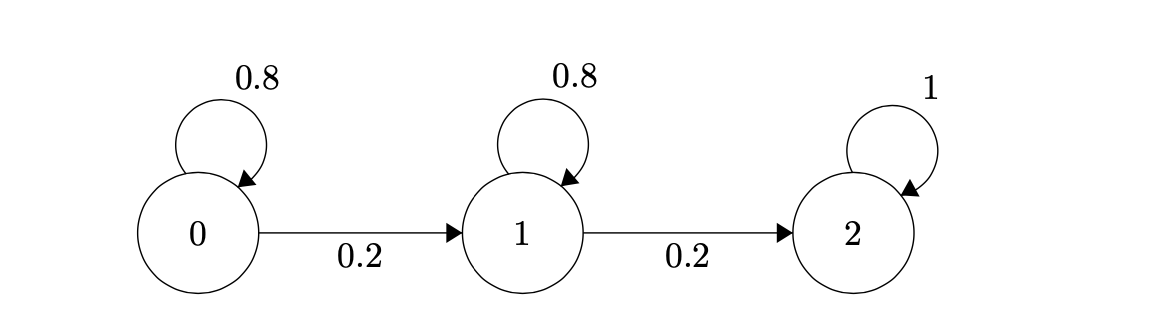
\includegraphics[scale=0.5]{t6.png}
        \end{center}
    \end{figure}
    Notice that at state 0, the chain has $P=0.8$ to stay the same, $P=0.2$ to transfer to state 1. 
    So state 0 and state 1 are not recurrent. At state 1, the chain has $P=0.8$ to stay the same, 
    and $P=0.2$ to transfer to state 2 and stay in state 2 forever. Notice that state 2 is an absorbing state, 
    and once it leaves 0 or 1, it can not go back. \\
    Consider the following story: One person at state 1, and do some work with $P=0.8$ fail, and $P=0.2$ success. 
    Once he successfully done this work, he moves to state 2, and do the same work again, once he succeed again, 
    he will stop. We define $t_0$ be the time he finished the first work, and $t_1$ be the time he finished the second work. 
    It's obviously that for each work, the time of his first success follows First Success distribution
    (i.e. Geometric Distribution), with parameter $0.2$ ($t_{0,1} \sim Geom(0.2)$).\\
    Hence,
    $$E(T) = E(t_0) + E(t_1) = 2\cdot \frac{1}{p} = 10$$
    and 
    $$Var(T) = Var(t_0) + Var(t_1) = 2\cdot \frac{1-p}{p^2} = 40$$
\end{homeworkProblem}


\begin{homeworkProblem}
    \textbf{Solution}
    \begin{enumerate}
        \item [a)]
            If the chain returns to state 1, it must go to state 2 (with probability $0.5$), and then return to state 1 
            (with probability $0.5$), and once it leaves state 1 and 2, it will never return to state 1.
            So, $P(N=0) = 0.5\cdot 0.5 = 0.25$, for it first goes to state 2, then goes to state 3, never returns back.
            And for all $N = 0,1,2,\ldots, k$. Suppose it runs to state 1 and 2 $l$ times in total. From $k+l$ places 
            choose $2l$ of them and say on this steps the chain runs from $state_1$ to $state_2$, other times, it remains on $state_1$, 
            We have:
            $$P(N=k) = 0.25\cdot \sum_{l=0}^{k}{\binom{k+l}{2l} (\frac{1}{2})^{k+l}}$$
        \item [b)]
            In this problem, we only need to consider state 3,4,5 and 6, ignoring state 1 and 2. The new Markov chain is 
            inreducible, and have stationary distribution. Notice that the transition matrix $Q$ is symmetric (i.e. $q_{ij} = q_{ji}$), 
            the stationary distribution is reversible. Hence, 
            $$s_3 = \frac{1}{4}$$
            So, the fraction of the time that the chain spend in state 3 is $\frac{1}{4}$.
    \end{enumerate}
\end{homeworkProblem}

\begin{homeworkProblem}
    \textbf{Solution}
        \begin{enumerate}
            \item [FDM] Queue\\
            For this system structure, we consider each subsystem.
            Define $\rho = \frac{\lambda}{k\mu}<1$\\
            The mean number of customers in subsystem: $E(N) = \sum_{i=0}^{\infty}{i\pi_i} = \frac{\rho}{1-\rho}$\\
            The mean number of customers in each queue: $E(N_q) = \sum_{i=0}^{\infty}{(i-1)\pi_i} = \frac{\rho^2}{1-\rho}$\\
            Mean time in system: $E_t =  \frac{1}{\mu - \lambda/k} = \frac{k}{k\mu - \lambda}$\\
            Mean time in queue: $E_{tq} = E_t - \frac{1}{\mu} = \frac{\rho}{\mu - \lambda/k} = \frac{\lambda}{k\mu^2 - \lambda\mu}$\\
            - Pros: When input are many independent tasks, it will handles well. The best case is, each queue has the same length, 
            the overload is balanced. In this case, data processing is parallized, the efficiency same as M/M/1 queue.\\
            - Cons: If the overload is not balanced (i.e. One queue is extremely long, while other servers are idle). In this case, 
            this model retrogrades to a single queue with parameter $\lambda$ and $\mu/k$, the efficiency is very low.

            \item [M/M/1] Queue\\
            Define $\rho = \frac{\lambda}{k\mu}<1$\\
            The mean number of customers in subsystem: $E(N) = \sum_{i=0}^{\infty}{i\pi_i} = \frac{\rho}{1-\rho}$\\
            The mean number of customers in each queue: $E(N_q) = \sum_{i=0}^{\infty}{(i-1)\pi_i} = \frac{\rho^2}{1-\rho}$\\
            Mean time in system: $E_t =  \frac{1}{k\mu - \lambda} $\\
            Mean time in queue: $E_{tq} = E_t - \frac{1}{k\mu} = \frac{\rho}{k\mu - \lambda} = \frac{\lambda}{k^2\mu^2 - k\lambda\mu}$\\
            - Pros: Unlike FDM model, the worst case will never happen, it's stable, and we don't need to consider overload balancing. 
            It will always has the same expectation of queuing time and processing time.\\
            - Cons: In real systems, it's hard to implement such a single system with high throughput.

            \item [M/M/k] Queue\\
            The markov chain of M/M/k model is shown below:
            \begin{figure}[H]
                \begin{center}
                    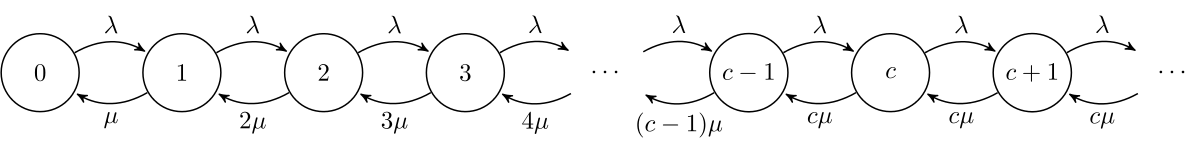
\includegraphics[scale=0.3]{mmk.png}
                \end{center}
            \end{figure}
            In the M/M/k queue, also define $\rho=\frac{\lambda}{k\mu}<1$, 
            \begin{align}\nonumber
                p_{m} = 
                \begin{cases}
                    p_{0}\prod\limits_{i=0}^{m-1}\frac{\lambda}{(i+1)\mu}=p_{0}(\frac{\lambda}{\mu})^{m}\frac{1}{m!}, \quad m<k \\
                    p_{0}\prod_{i=0}^{k-1}\frac{\lambda}{(i+1)\mu}\prod\limits_{j=0}^{m-1}\frac{\lambda}{k\mu}=p_{0}(\frac{\lambda}{\mu})^{m}\frac{1}{k!k^{m-k}}, \quad m\geq k
                \end{cases}
            \end{align}
            where $p_{0}=[\sum\limits_{m=0}^{k-1}\frac{(k\rho)^{m}}{m!}+\sum\limits_{m=k}^{\infty}\frac{(k\rho)^{m}}{k!k^{m-k}}]^{-1}=[\sum\limits_{m=0}^{k-1}\frac{(k\rho)^{m}}{m!}+\frac{(k\rho)^{k}}{k!(1-\rho)}]^{-1}$ 
            since $\sum\limits_{m=0}^{\infty}p_{m}=1$\\
            Then, we calculate the expected number of customers in the system.
            \begin{equation}\nonumber
                E(N)=\sum\limits_{m=0}^{\infty}mp_{m}= \frac{(k\rho)^{k}\rho p_{0}}{k!(1-\rho)^{2}} + k\rho
            \end{equation}
            For we know the total traffic intensity 
            $$p_i=\frac{p_{0}(k\rho)^{k}}{k!}$$
            We can obtain: 
            \begin{equation}\nonumber
                p_{q}=\sum\limits_{m=k}^{\infty}p_{m}=\frac{p_{i}}{1-\rho}=\frac{(k\rho)^kp_{0}}{(1-\rho)k!}
            \end{equation}
            Then, the mean number of customers in queue is 
            $$E(N_q)=p_{0}\frac{(k\rho)^{k}}{k!}\sum\limits(m-k)\rho^{m-k}=p_{0}\frac{(k\rho)^{k}}{k!}\sum\limits_{n=0}^{\infty}n\rho^{n}$$
            Hence, 
            \begin{eqnarray}\nonumber
                E(N_q)=\frac{\rho}{1-\rho}p_{q}
            \end{eqnarray}
            By little's law,
            \begin{equation}\nonumber
                \begin{aligned}
                    E_t & = \frac{\rho p_{q}}{\lambda(1-\rho)}\\
                    E_{tq} & = E_t+\frac{1}{\mu}=\frac{1}{\mu}+\frac{p_{q}}{k\mu-\lambda}
                \end{aligned}            
            \end{equation}

            Since $E_t(M/M/k)=\frac{1}{\mu}+\frac{p_{q}}{k\mu-\lambda}$, and $E_t(M/M/1)=\frac{1}{k\mu-\lambda}$. \\
            Under light load ($\rho\ll 1$),  $p_{q}\to 0$, we will get $\frac{E_t(M/M/k)}{E_t(M/M/1)} \approx k$\\
            Under heavy load ($\rho\rightarrow1$), $p_{q}\to 1$ and $\frac{1}{\mu}\ll\frac{1}{k\mu-\lambda}$, 
            we will get $\frac{E_t(M/M/k)}{E_t(M/M/1)}\approx 1$.\\
            So we can analyze the pros and cons:\\
            - Pros: Under heavy load, its performance is the same as the M/M/1 queue, the performance is relative high.\\
            - Cons: Under light load, it will have a pretty poor performance, at most $k$ times slower than M/M/1 queue.
        \end{enumerate}
\end{homeworkProblem}


\end{document}
